\documentclass[12pt]{article}
\usepackage{graphicx}
\graphicspath{ {./fig/} }

\title{ \textbf{EE230: Homework-2\\
Plotting and Data Analysis Exercise}}

\author{Prateek Garg, 20D070060}

\begin{document}
\noindent
\maketitle


\section{Overview of the experiment}

\subsection{Aim of the experiment}
To plot current versus voltage in a semilog graph from given current voltage characteristics and obtain ideality factor "$n$" by visual inspection of semi-log graph.
\subsection{Methods}
"$n$" is defined in the following equation $$I = I_{o}(e^{\frac{qV}{nk_{B}T}}-1)$$
$k_{B}$ = Boltzmann constant, $T$ = temperature, $q$ = elementary
charge. \\
$I$ = current, $I_{o}$ = reverse saturation current, $V$ = applied voltage
Taking logarithm on $I$, we get 
$$ln(I) = ln(I_{o}(e^{\frac{qV}{nk_{B}T}}-1)),$$ 
$$ln(I) = ln(I_{o})+ln(e^{\frac{qV}{nk_{B}T}}-1),$$
$$ln(I) = ln(I_{o})+\frac{qV}{nk_{B}T}+ln(1-e^{\frac{-qV}{nk_{B}T}}),$$

As V becomes large, $e^{\frac{-qV}{nk_{B}T}} \rightarrow 0$ so $ln(1-e^{\frac{-qV}{nk_{B}T}}) \approx ln(1)=0$ \\
So when V is large enough
$$ln(I) = ln(I_{o})+\frac{qV}{nk_{B}T}$$

\section{Design}
Taking two points $V_{1}$ and $V_{2}$ we can estimate n. 
$$ln(I_{1})-ln(I_{2}) = \frac{q(V_{1}-V_{2})}{nk_{B}T}$$
$$n=\left(\frac{q}{k_{B}T}\right)\cdot \left(\frac{V_{1}-V_{2}}{ln(I_{1})-ln(I_{2})}\right)$$
$k_{B}$ = Boltzmann constant, $T$ = temperature, $q$ = elementary
charge. \\

\section{Simulation results}
\makebox[\textwidth]{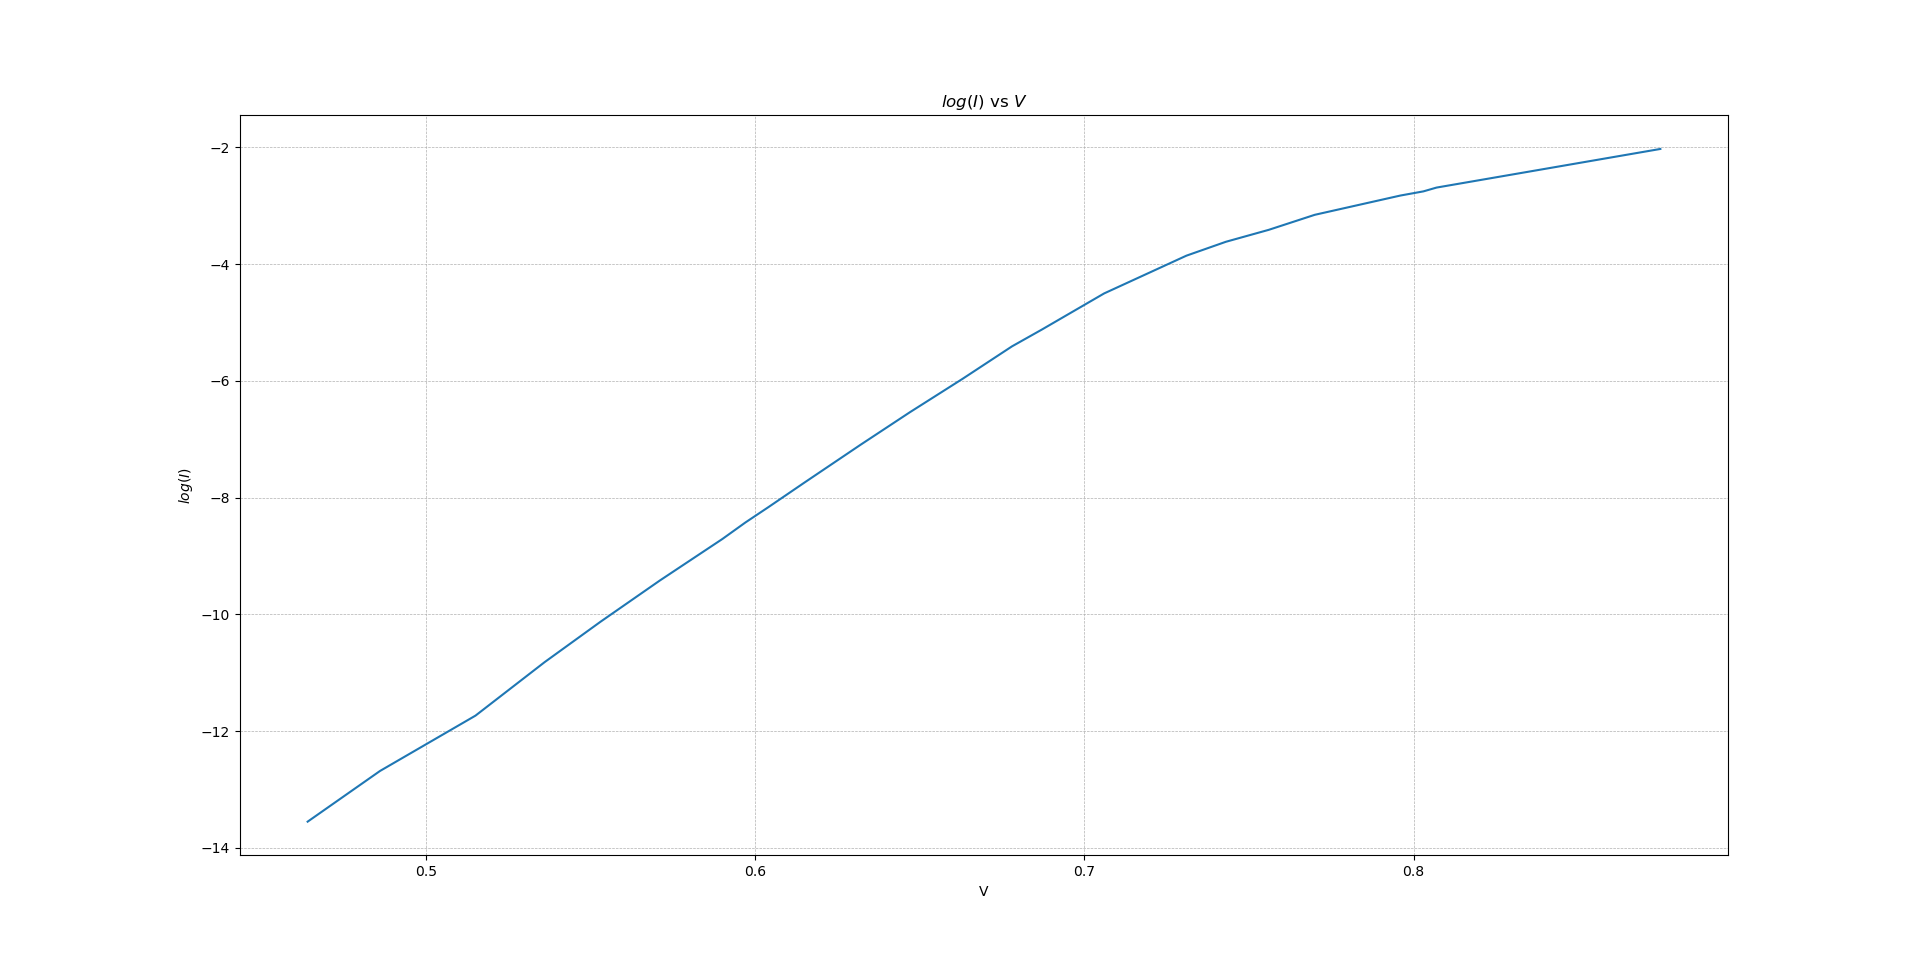
\includegraphics[width=\paperwidth]{Figure_1.png}}

\section{Experimental results}
Taking last 2 values from the dataset,\\
$(V_{1},I_{1})=(0.807,0.0681)$ and $(V_{2},I_{2})=(0.875,0.132)$ \\
$T=300K,$ $q=1.6 \times 10^{-19} C$ $k_{B}=1.38\times10^{-23}$ \\
and using them in the derived expression we get, $$n=3.95$$
\section{Experiment completion status}
All the sections were completed.
\end{document}
